
\begin{center}
	\Huge
	Vektorfunktioner
\end{center}
\section*{Definition af vektorfunktion}
\stepcounter{section}

Nyt emne; vektorfunktioner. Vektorfunktioner er funktioner af én variabel hvis dispositionsmængde består af vektorer. Vi har allerede stiftet bekendtskab med en type vektorfunktion; linjens parameterfremstilling. Hvis vi har en retningsvektor $\vv{r}$ og et punkt $P(x_0,y_0)$ som linjen skærer igennem har vi set at linjens parameterfremstilling er givet ved
\begin{align*}
	l:\ \begin{pmatrix} x \\ y
	\end{pmatrix} =
	\begin{pmatrix}
	x_0 \\ y_0
	\end{pmatrix} +t
	\begin{pmatrix}
	r_1 \\ r_2
	\end{pmatrix}.
\end{align*}
Vil vi repræsentere denne som en vektorfunktion kan vi skrive
\begin{align*}
	\vv{r}(t) = \begin{pmatrix} x \\ y
	\end{pmatrix} =
	\begin{pmatrix}
	x_0 + tr_1 \\
	y_0+tr_2
	\end{pmatrix},
\end{align*}
og $\vv{r}$ er nu en funktion af $t$. Vi skriver som tidligere $\vv{r}: \mathbb{R} \to \mathbb{R}^2$. Vi vil definere en vektorfunktion mere præcist:

\begin{defn}[Vektorfunktion]
	En funktion $\vv{r} : \mathbb{R} \to \mathbb{R}^2$ givet ved
	\begin{align*}
		\vv{r}(t) = 
		\begin{pmatrix}
			x(t) \\ y(t)
		\end{pmatrix}
	\end{align*}
	kaldes en \textit{vektorfunktion}.
	Funktionerne $x$ og $y$ kaldes for vektorfunktionens \textit{koordinatfunktioner}.
\end{defn}
Grafen for en vektorfunktion kaldes ofte for en \textit{parameterkurve}, og vektorfunktionen er denne kurves \textit{parameterfremstilling.} 

\begin{exa}
	Vi vil ofte tænke på vektorfunktioner som funktioner, der beskriver placeringen af en partikel i planen. Hvis en partikel bevæger sig langs en kurve i planen, så vil 
	parameterfremstillingen for denne kurve en vektorfunktion $\vv{r}$, og tilsvarer partiklens stedvektor. Parameterkurven vil i dette tilfælde kaldes for \textit{banekurven}. 
\end{exa}

\begin{exa}
	Lad os betragte vektorfunktionen $\vv{r}:\mathbb{R} \to \mathbb{R}^2$ givet ved
	\begin{align*}
		\vv{r}(t) = \begin{pmatrix}
			t^2-10\\
			t^2+2t-1
		\end{pmatrix}
	\end{align*}
	Vi kan tegne denne i Maple ved at skrive 
	\begin{align*}
		&\texttt{with(Gym):}\\
		&\texttt{r(t):= <t\string^2-10,t\string^2+2t-1>}\\
		&\texttt{vektorPlot(r(t))}
	\end{align*}
	Vi får så følgende plot
	\begin{center}
		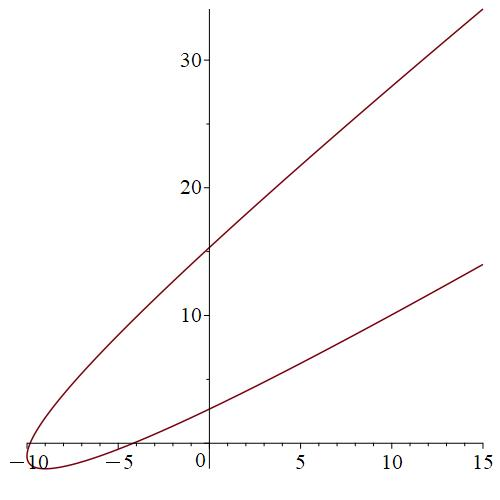
\includegraphics[width=0.7\textwidth]{Billeder/vektor1.jpg}
	\end{center}
	Vi kan specificere akserne og t-intervallet ved at skrive
	\begin{align*}
		\texttt{vektorPlot(r(t), t = -7 .. 7, view = [-15 .. 15, -5 .. 15])}.
	\end{align*}
	Dette giver følgende plot
	\begin{center}
		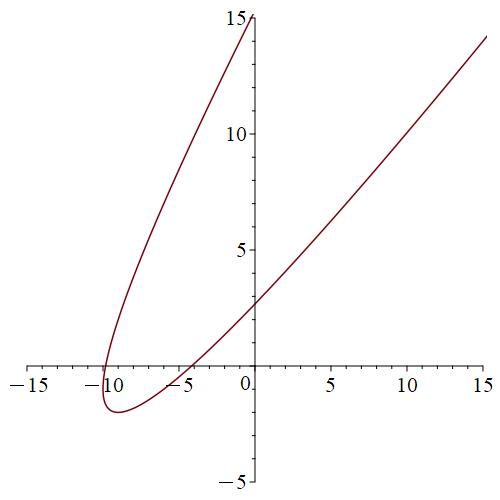
\includegraphics[width=0.7\textwidth]{Billeder/vektor2.jpg}
	\end{center}
\end{exa}

\begin{exa}
	Vi betragter igen $\vv{r}:\mathbb{R} \to \mathbb{R}^2$ givet ved
	\begin{align*}
		\vv{r}(t) = 
		\begin{pmatrix}
			t^2-10 \\
			t^2+2t-1
		\end{pmatrix}.
	\end{align*}
	Hvis vi ønsker at bestemme koordinaterne til et givent $t$, så indsættes dette blot i koordinatfunktionen. Lad os bestemme $\vv{r}(2)$.
	\begin{align*}
		\vv{r}(2) =
		\begin{pmatrix}
			2^2-10 \\
			2^2+2\cdot 2 -1
		\end{pmatrix}
		=
		\begin{pmatrix}
			-6 \\
			7
		\end{pmatrix}.
	\end{align*}
\end{exa}

\section*{Skæring med akser}
\stepcounter{section}

Vi kan for vektorfunktioner være interesseret i, hvornår de skærer akserne. For at bestemme skæringen med $x$-aksen for parameterkurven for en vektorfunktion 
\begin{align*}
	\vv{r}(t) = 
	\begin{pmatrix}
		x(t)\\
		y(t)
	\end{pmatrix}
\end{align*}
løses ligningen $y(t)=0$. Løsningen $t_0$ indsættes så i vektorfunktionen og skæringspunktets koordinater vil da være
\begin{align*}
	\vv{r}(t_0) = 
	\begin{pmatrix}
		x(t_0) \\
		0
	\end{pmatrix}.
\end{align*} 
Skal skæringspunktet med $y$-aksen findes sættes koordinatfunktionen $x(t)$ tilsvarende lig $0$. 

\begin{exa}
	Vi betragter nu $\vv{r}:\mathbb{R} \to \mathbb{R}^2$ givet ved
	\begin{align*}
		\vv{r}(t) = 
		\begin{pmatrix}
			t^2-4 \\
			t^2-6t+9
		\end{pmatrix}.
	\end{align*}
	Skal skæringspunkterne med $x$-aksen findes løses ligningen
	\begin{align*}
		y(t) = t^2-6t+9 = 0,
	\end{align*}
	hvilket vi kan løse med diskriminantformlen og får løsningerne 
	\begin{align*}
		t_0 = 3
	\end{align*}
	Dette indsættes i koordinatfunktionen $x(t)$:
	\begin{align*}
		x(3) = 3^2-4 = 5
	\end{align*}
	Derfor har parameterkurven for $\vv{r}$ én skæring med $x$-aksen i punktet $(5,0)$.
	Skal vi tilsvarende finde skæringspunkterne med $y$-aksen sættes koordinatfunktionen $x$ lig 0, og vi får:
	\begin{align*}
		x(t) = t^2-4=0,
	\end{align*}
	hvilken har løsningerne 2 og $-2$. 
	Dette indsættes i koordinatfunktionen $y$, og vi får
	\begin{align*}
		y(2) = 2^2-6\cdot 2+9 = 1
	\end{align*}
	og 
	\begin{align*}
		y(-2) = (-2)^2 -6(-2) + 9 = 25.
	\end{align*}
	Derfor har vi desuden skæringspunkterne med $y$-aksen $(0,1)$ og $(0,25)$. Vi tegner parameterkurven i Maple og får følgende plot.
	\begin{center}
		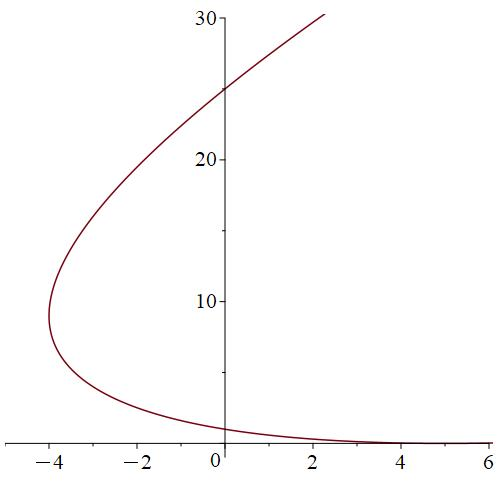
\includegraphics[width=0.7\textwidth]{Billeder/vektor3.jpg}
	\end{center}
	Det ser af grafen ud til, at vi har fundet de korrekte skæringspunkter med akserne.
\end{exa} 
\section*{Opgave 1}

\begin{enumerate}[label=\roman*)]
	\item En vektorfunktion er givet ved
	\begin{align*}
		\vv{r}(t) = 
		\begin{pmatrix}
			t+4 \\
			2t+5
		\end{pmatrix}.
	\end{align*}
	Bestem $\vv{r}(-1)$ og $\vv{r}(1)$, og tegn parameterkurven for $\vv{r}$ i Maple. Hvilken vej bevæger $\vv{r}$ sig, når $t$ vokser?
	\item En vektorfunktion er givet ved
	\begin{align*}
		\vv{r}(t) = 
		\begin{pmatrix}
			t^2-t-1 \\
			-2t^2+2t+4
		\end{pmatrix}.
	\end{align*}
	Bestem $\vv{r}(3)$ og $\vv{r}(4)$, og tegn parameterkurven for $\vv{r}$ i Maple. Hvilken vej bevæger $\vv{r}$ sig, når $t$ vokser?
	\item En vektorfunktion er givet ved
	\begin{align*}
		\vv{r}(t) = 
		\begin{pmatrix}
			t^5-1 \\
			t^3+2t^2+4
		\end{pmatrix}.
	\end{align*}
	Bestem $\vv{r}(-1)$ og $\vv{r}(2)$, og tegn parameterkurven for $\vv{r}$ i Maple. Hvilken vej bevæger $\vv{r}$ sig, når $t$ vokser?
\end{enumerate}

\section*{Opgave 2}
Bestem skæringen med $x$ og $y$-akserne for følgende vektorfunktioner
\begin{align*}
	&1) \ \vv{r} = 
	\begin{pmatrix}
		2t -2 \\
		5t-10
	\end{pmatrix}
	&&2) \ \vv{r} = 
	\begin{pmatrix}
		t^2-1 \\
		t-2
	\end{pmatrix} \\
	&3) \ \vv{r} = 
	\begin{pmatrix}
		t-10 \\
		t^2-6t-12
	\end{pmatrix}
	&&4) \ \vv{r} = 
	\begin{pmatrix}
		t^4-1 \\
		t^6-t^4+t^2+2t+2
	\end{pmatrix} \\
	&5) \ \vv{r} = 
	\begin{pmatrix}
		\sqrt{t}-2 \\
		-3t^3+6t-9
	\end{pmatrix}
	&&6) \ \vv{r} = 
	\begin{pmatrix}
		\ln(t) \\
		\sqrt{t} \\
	\end{pmatrix}
\end{align*}